\documentclass[a4paper]{report}
\usepackage[utf8]{inputenc}
\usepackage[english]{babel}
\usepackage{hyperref}
\usepackage{a4wide}
\usepackage{algorithm2e}
\usepackage{siunitx}

\hypersetup{pdftitle={Sistema de Gestão de Vendas},
pdfauthor={Filipe Felício, Henrique Ribeiro, João Correia},
colorlinks=true,
urlcolor=blue,
linkcolor=black}
\usepackage{subcaption}
\usepackage[cache=false]{minted}
\usepackage{listings}
\usepackage{booktabs}
\usepackage{multirow}
\usepackage{appendix}
\usepackage{tikz}
\usepackage{authblk}
\usetikzlibrary{positioning,automata,decorations.markings}

\begin{document}

\title{Sistema de Gestão de Vendas\\ 
\large Grupo Nº 39}
\author{Filipe Felício (A85593) \and Henrique Ribeiro(A89582) \and João Correia (A84414)}
\date{\today}

\begin{center}
    \begin{minipage}{0.75\linewidth}
        \centering
        
\includegraphics[width=0.4\textwidth]{eng.jpeg}\par\vspace{1cm}
        \vspace{1.5cm}
        \href{https://www.uminho.pt/PT}
        {\color{black}{\scshape\LARGE Universidade do Minho}} \par
        \vspace{1cm}
        \href{https://www.di.uminho.pt/}
        {\color{black}{\scshape\Large Departamento de Informática}} \par
        \vspace{1.5cm}
        \maketitle
    \end{minipage}
\end{center}

\tableofcontents

\pagebreak

\chapter{Introduction}



The following pages serve the purpose of in-depth reviewing the sophistication of our software implementation
of a modular Sales Management System that is capable of processing sales data in a large scale, 
whilst also being able to quickly provide products and clients info, and answer
multiple questions and challenges with optimal solutions.

With the key word on the last paragraph being \textit{sophistication}, this report shall sustain the thesis 
of our choices in terms of Algorithms, Data Structures and Architecture being the most effective, reliable 
and appropriate, within each of the singular queries and their spot in the overall plain of the program, 
according to the fitting metrics of development. 

In order to achieve peak performance in a multi-variable set of goals, such as time, scalability , encapsulation and
memory use, this study will reflect the potential of our own approach to solve the given task with logical allocation of resources to give the best overall experience to a user of this application, given that on a micro dissection not all the choices were optimal we aim at the highest degree of optimization at the amortized
macro analyses.

\chapter{Problem interpretation and challenges}\label{chap:Problem interpretation and challenges}

The proposed project was to develop a sales management system (SGV) capable of emulating a mid sized business. There are three files that detail the emulated environment, they are:

\begin{itemize}
    \item A file containing Clients' IDs;
    \item A file containing Products' IDs;
    \item A file describing sales information containing the ID of the bought product, the ID of the client who bough it, the price of an unit, the number of units bought, if the product was bought normally or through a sale and in which branch it was bought;
\end{itemize}
The system must also be able to answer 13 different queries, these are as follows:
\begin{enumerate}
    \item Read the files referenced above, checking if the entries are valid and then process the information, loading it in it's data structures.
    \item List all the products whose IDs start by a user provided character.
	\item Given a product's ID and a month, return the number of sales and the total value billed for that product. The user must decide if he wants to see the results grouped globally or discriminated by branch
    \item Return a list of products which were never bought, alphabetically ordered  by their ID. The user can decide if he wants to check globally or by branch. 
    \item Return a list of clients who made purchases in all branches, also alphabetically ordered  by their ID.
    \item Determine the number of clients who never bought anything, as well as the number of products which were never bought.
    \item Given a client's ID, create a table a table with the number of products bought by that client. The table must be divided by month and branch.
    \item Determine the number and value of the sales that happened between a defined month interval.
    \item Given a product's ID and a branch number, list the ID's of the clients who bought it, distinguishing them by if the client  bought it normally or bought it at a discount.
    \item Given a client's ID and a month, list the ID's of the products he bought more units. The list must be ordered  by the number of units bought, in descending order.
    \item List the N most sold products during the whole year. For each product, the number of sales and clients of that product in each branch must also be presented.
    \item Given a client's ID, list the N products in which the client spent more money
    \item Show a summary of what happened in query 1. This summary must include the path of each file read, as well as the number of lines read and the number of lines which were valid.
\end{enumerate}

The main purpose of this project, as we understood it, was to learn the best practices of developing scalable mid-to-large scale software while keeping in mind crucial design principles, such as encapsulation and modularity.

One of the main challenges was the process of choosing the data structures, since it demanded a careful and methodical approach, as detailed on chapter \ref{chap:data structures}.


\chapter{Project  architecture and Modules}\label{chap:api}
The project adopts the \textit{MVC} (Model, View,
Controller) architecture. 
A dependency diagram of our program can be found on attachment \ref{img:dependency graph}.
The details of each layer are exposed below.
\section{Model} 
The model is the part of the software responsible for inserting, managing and manipulating data.
In our program the modules that constitute the model are explained below, being the interface module the
main module, since it is the one who encapsulates all the other ones.

\subsection{Client}
The Client module is responsible for holding information and answering simple 
questions regarding a single client, such as its id and if and where he has bought something.

\subsection{Clients}

This module is responsible for storing all the clients.
The data structure used for this purpose was an hash table, provided by the GLib library.
The reasons for why this was the chosen data structure are later presented 
on chapter \ref{chap:data structures}.

\subsection{Product}

The product module holds information about a product, such as its id and where the product was bought.
It has an API that is very similar to the Clients', being capable of answering simple questions.

\subsection{Products}

The module is responsible for storing all the products. Because it has been built
with scalability in mind, as with the Clients module,
it uses an Hash table for storing and retrieving data.

\subsection{Sales}

This module is responsible for holding the information about a product's billing and profits.
After researching the problem, the need for creating a module representing a single sale wasn't found,
so this module is the module directly responsible for answering information about the all the sales of a product,
namely the number of times it has been sold, the total amount of units sold and the total value
of sales of that product. This is done by using multi-dimensional arrays, 
using the indexes to separate information by month, branch and type of sale. 

\subsection{TotalSales}

This is the module for storing all the sales structures. As with the products
and clients modules, this one also uses an hash table. It will serve as a middleman 
for creating and updating sales information regarding a product whilst also providing functions to check if a sale is valid.
No reference to clients is present in this module as that is responsibility of the branch module.


\subsection{Branch}

This module is responsible for storing the information about the sales made in a certain
branch of our business. It is capable of establishing a relation between all the products a client bought in a certain
branch and all the clients who bought a product.
This is done by using plethora of structures who boil down to nested hash tables.
The first layer is composed of two hash tables. The first one, for each product, contains a second hash table for each
client who bought it. It then contains a structure with information about the client's purchases of that product in that branch.
The same logic is applied to the second pair of nested hash tables, which establish a relation between 
every client and all the products they have bought.


\subsection{Interface}

This is the module where the SGV is implemented. This structure will encapsulate all modules referenced above:
A products catalogue, a clients catalogue, a totalSales structure and an array of branches.
This module also contains all the interactive queries, therefore it will interact with the controller when the user requests information from the application.


\section{Controller}

This is the layer responsible for interaction with the user. It calls the View layer to present the options that the user may call. 
After an option is chosen, the Controller will then communicate with the Model layer to either change the internal
representation of the data or to provide the answer to the chosen query.

\subsection{Controller}
This module implements functions capable of navigating our intricate View layer whilst also being responsible for validating the user’s input and handling the implemented queries, calling the  Model layer and obtaining the QueryOutput structure, which will be  used to present the query’s answer.

\section{View}
This layer is responsible for presenting formatted information to the user, through the 
use of tables, diagrams and other graphics. It will also be responsible for presenting large amounts of data in a format the user can easily navigate.

\subsection{View}

The view module presents the application's menu to the user with some imaginative techniques to provide an immersive, easy-to-use experience.
It will also present the user with the answers to all the queries in a navigable format, thus serving also as 
a String \textit{paginator}.



\section{Transversal modules}
These are the modules who will be used by more than one of the above layers
and, as such, cannot be labelled as one of them.

\subsection{QueryOutputs}
This module consists of a group of structures which will be used to return the answer's to the interactive queries. 
Although some queries could use the same structure to return their answers, we opted for implementing a different structure for each query. Doing so, it becomes easier to rewrite code in case we decide to change the way some query works or what information it will return.
\subsection{ProductInfo}
This module is used in query getTopSelledProducts() to keep track of a product's number of units bought and clients. Although it could be declared as an ancillary structure inside another module, for a reason of modularity and encapsulation, it was declared as different module altogether since it is called upon by several different modules.

\subsection{Config}
This module contains user defined macros for our program. The value of these macros can be
modified to increase or decrease the application's dimension, making it possible to attain software scalability 
without having to know how the software is implemented. Some examples of these macros 
are: the size of a client's and product's id, the number of different types of sales and the number 
of branches.  



\chapter{Data Structures }\label{chap:data structures}

When designing mid to large scale software, one of the most crucial decisions consists on which data structures to use in order to strike a balance between memory usage, speed and scalability.
As described on chapter \ref{chap:api}, both the clients module and the products module implement the glib version of Hash tables.
This choice was based in both analytical and empirical evidence, as shown below.
Two data structures seemed promising for our software, they were:
\begin{itemize}
    \item A Hash table
    \item An Array of 26 Balanced Trees
\end{itemize}
The program has two phases where the data structures are consulted or modified: When the information
is loaded to the data structures, right at the beginning of the program, and when answering the proposed queries.

While the Hash table's insertion and search time complexity is  $O(1)$, meaning it will have a stellar performance when inserting and validating information, it becomes less effective when sorting data, requiring the use of a sorting algorithm like the one used in the program,  \textit{qsort()}. The trees will be slower when inserting and validating data since their operations are $O(log n)$, but, due to their ordered insertion algorithm, will provide faster answers to queries where the answer must be ordered. 

To test both data structures, the products module was implemented both using an hash table (\textit{products.c}) and using an array of trees (\texttt{experimental\_code/productsTrees}). To measure the impact, three times were measured: the load time, the time to answer query 2 and query 4, these are the processes that are most impacted by what data structure is implemented. The results can be found on tables  \ref{tab:hashProductsBench} and  \ref{tab:treesProductsBench}.

As expected, the load time is faster and the second query is slower when using the Hash table, however, the fourth query is actually slower when using the tree array. This is due to a completely different reason than time complexities: the glib's API. The GHashTable API has a wider variety of functions when compared to the GTree API, which results in better optimizations when using functions such as \texttt{g\_hash\_table\_iter} and \texttt{g\_hash\_table\_get\_keys} that don't have any equivalents in the GTree API. This is another reason we decided to use Hash tables: it provides a better API for scalable software. We also see that as the program grows, the load time increases accordingly while the queries' answer time remains the same. If scalability is in one's best interest, the use of hash tables  comes as the most sensible choice, since it provides a better load time while sacrificing little in query time.




\chapter{Performance metrics}

When developing software, there are a myriad of different metrics that can be used to evaluate its performance. In the context of this project, while having in mind the specification detailed on chapter \ref{chap:Problem interpretation and challenges}, the aspects we found more relevant to measure were memory management and execution time, with a special emphasis on the first one, since our application is not aided by databases.



\section{Memory management}

As referenced above, the program does not use databases, which means that all the data must be loaded to memory. With this concern, we developed the application with the goal of being able to still fit large amounts of data. That means that we programmed our modules to make use of the heap, since the stack has limited size. While sacrificing some speed in the load process, this ensures our application is capable of handling bigger amounts of data.


One of the greatest risks associated with this kind of approach when programming in C is the threat of memory leaks.
The problem with memory leaks is the fact that a program can run with these errors whilst appearing to execute normally and producing the expected results.



\section{Memory usage}

In order to check our program for memory leaks, the \textit{Valgrind} tool was used. No memory leaks were found, except for 18,612 bytes which came Glib. These were completely unavoidable as the very own act of simply including the glib header file caused them.

Not only does \textit{Valgrind}  warn of memory leaks, it also informs the user of the specific parts of the software that cause these issues.
This tool was very useful, especially when used alongside \textit{GDB}, when it came to debbuging.

With the use of the \textit{memusage} tool, we are able to verify the max amount of data allocated in the heap for each sales document read.
From the \ref{img:memusage} graph, we can see that for 1 million sales the max amount of allocated memory were 339 MB.
From the \ref{img:memusage_3M} and \ref{img:memusage_5M} graphs, we can see that the max amount of allocated memory was 625 and 880 Mb, for 3 and 5 million sales, respectively. This demonstrates the effectiveness of our careful memory management, as memory usage grows sub linearly to the growth in the number of sales.


\section{Execution time}

Another issue will be the potential mishandling of data structures by programmers, since data structures such as Hash tables or binary trees may be poorly implemented, or, in the case of structures like Fibonacci heaps, might not match their theoretical performance in a practical setting.

It is crucial then, to test our use of these data structures to make sure our performance matches these structures' theoretical level of efficiency and run time.

We used the the \textit{time.h} library to evaluate the time it took for our queries to execute. These results can be seen in the \ref{tab:benches} table.

\chapter{Conclusion}
In conclusion, all the proposed queries are implemented efficiently with execution times that don't  worsen as data size increases. 

Managing to reduce the execution time for the queries whilst maintaining a small program load time would be a challenge worth pursuing.

Another challenge would be to implement our own version of the data structures instead of the ones provided by GLib, seeing as they could be better equipped to handle the specific problems of our SGV system since we would be able to fully customize them in what way we would see fit.

Trying to implement data bases in our program would also be of our interest as it would allow the application to scale exponentially more since it would not be bound by the RAM size of the computer running it.

\appendix
\chapter{Dependency Graph}
\begin{figure}[H]
    \begin{center}
        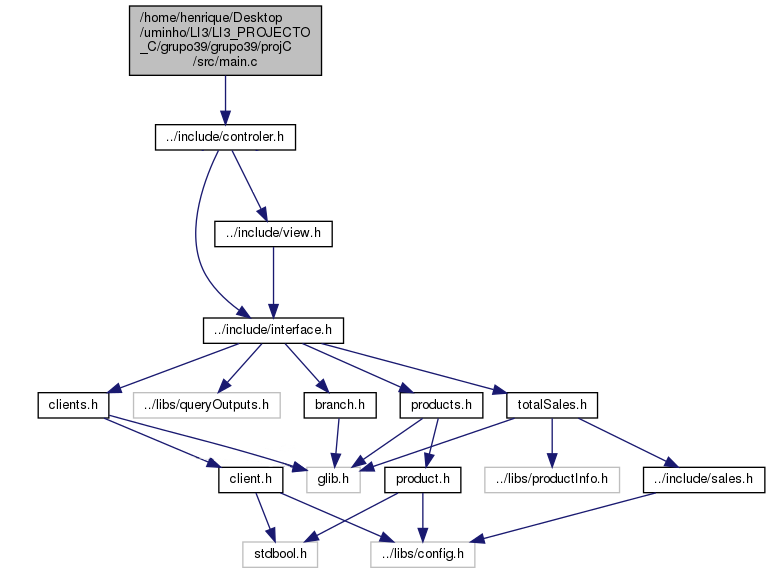
\includegraphics[width=1\textwidth]{dependency.png}\par
        \caption{Dependecy graph of the project.}
        \label{img:dependency graph}
    \end{center}
\end{figure}

\chapter{Memory usage graphs}
\begin{figure}[H]
    \begin{center}
        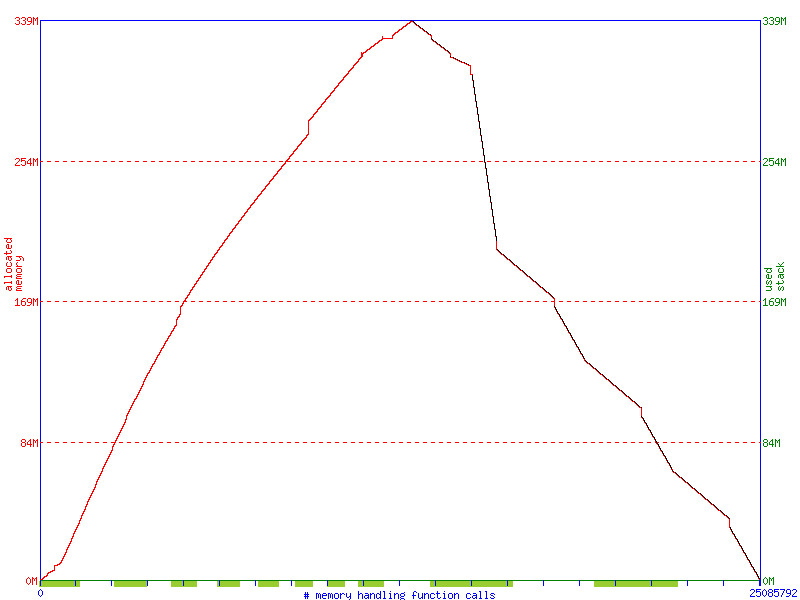
\includegraphics[width=1\textwidth]{memusage.png}\par\vspace{1cm}
        \caption{Graph depicting memory use for 1 million sales.}
        \label{img:memusage}
    \end{center}
\end{figure}

\begin{figure}[H]
    \begin{center}
        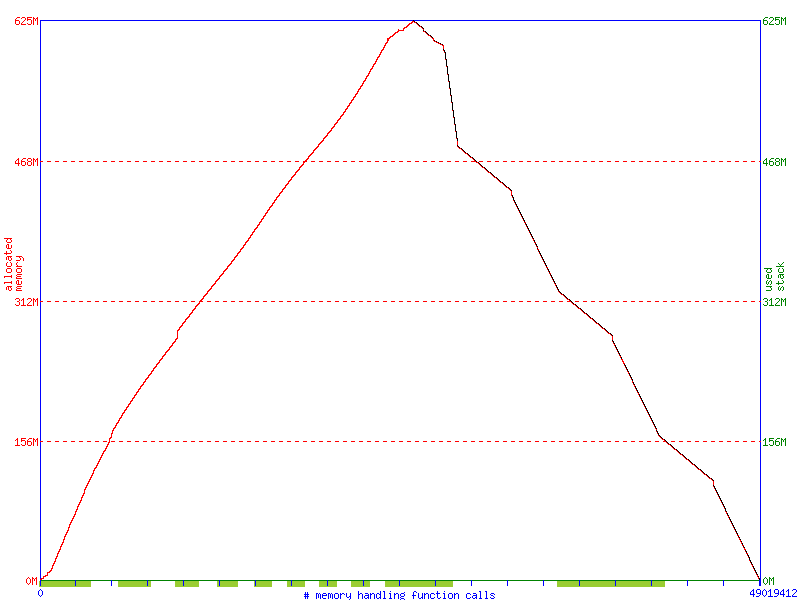
\includegraphics[width=1\textwidth]{memusage_3M.png}\par\vspace{1cm}
        \caption{Graph depicting memory use for 3 million sales.}
        \label{img:memusage_3M}
    \end{center}
\end{figure}

\begin{figure}[H]
    \begin{center}
        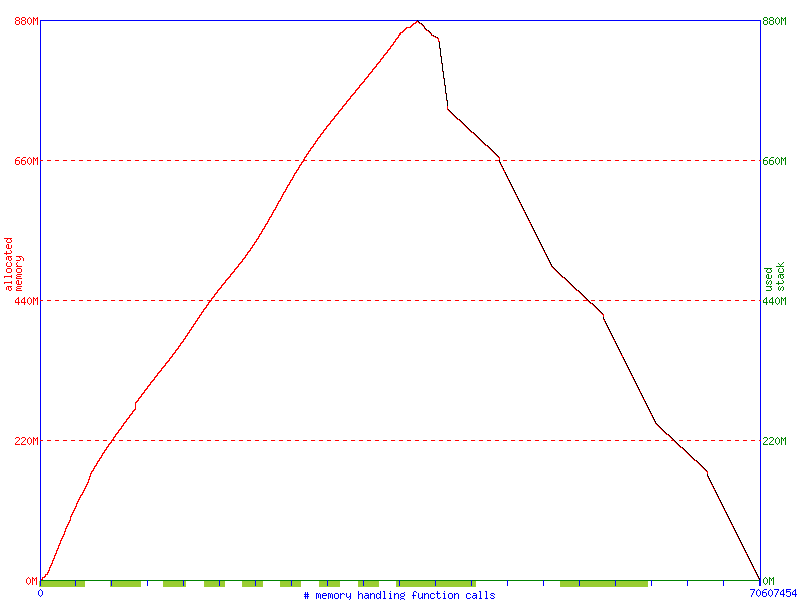
\includegraphics[width=1\textwidth]{memusage_5M.png}\par\vspace{1cm}
        \caption{Graph depicting memory use for 5 million sales.}
        \label{img:memusage_5M}
    \end{center}
\end{figure}

\chapter{Different products module implementations time tables}

\begin{table}[H]
    \begin{center}
        \begin{tabular}{| c | c | c | c |}
            \hline
            & 1 Million & 3 Millions & 5 Millions \\
            \hline
            Load Time & \num{2.66} & \num{9.10} & \num{15.72}  \\
            \hline
            Query 2 & \num{4.4e-3} &\num{4.4e-3} & \num{4.4e-3} \\
            \hline
            Query 4 &  \num{1e-2} &  \num{1.2e-2} &  \num{1.2e-2} \\
            \hline

        \end{tabular}
        \caption{Time  (in seconds)when the products module is implemented using an Hash table}
        \label{tab:hashProductsBench}
    \end{center}
\end{table}

\begin{table}[H]
    \begin{center}
        \begin{tabular}{| c | c | c | c |}
            \hline
            & 1 Million & 3 Millions & 5 Millions \\
            \hline
            Load Time & 3.94 & 11.55 & 21.22 \\
            \hline
            Query 2 &  \num{1.1e-3} &  \num{1.1e-3} &  \num{1.1e-3} \\
            \hline
            Query 4 &  \num{1.8e-2} &  \num{1.8e-2} &  \num{1.8e-2} \\
            \hline

        \end{tabular}
        \caption{Time  (in seconds)when the products module is implemented using an array of 26 AVL trees}
        \label{tab:treesProductsBench}
    \end{center}
\end{table}

\chapter{Application's time table}
\begin{table}[H]
    \begin{center}
        \begin{tabular}{| c | c | c | c | c |}
            \hline
            &  Input & 1 Million & 3 Million & 5 Million\\
            \hline
            Load Time  & --- & \num{2.66} & \num{9.10} & \num{15.72} \\
            \hline
            Query 2 & letter: "I"  & \num{2,91E-3} &  \num{3,03E-3} &  \num{3.04e-3}  \\
            \hline
            Query 3  & productID: "AF1184", month: 6   &  \num{1,10E-5} &	 \num{1,90E-5} &  \num{1,80E-5}\\
            \hline 
            Query 4  &  branchId:0 (all branches) &  \num{9,71E-3} &	 \num{8,80E-3} &  \num{9,28E-3} \\
            \hline
            Query 5 &  ---  &  \num{3,62E-3} &	 \num{3,81E-3} &  \num{3,74E-3}\\
            \hline
            Query 6  &  --- &  \num{7,52E-3} &	 \num{8,95E-3} &  \num{6,93E-3}\\
            \hline
            Query 7 &  clientID: "Z5000" &  \num{6,00E-6} &	 \num{4.00E-6} &  \num{7,00E-6}  \\
            \hline
            Query 8  &  minMonth: 1, maxMonth: 12 &  \num{1,00E-6} & \num{1,00E-6} &	 \num{1,00E-6} \\
            \hline
            Query 9  & productID: "AF1184", branch: 1 &  \num{1,50E-5} &	 \num{2.00E-5} &  \num{4,90E-5}\\
            \hline
            Query 10 & clientID: "Z5000", month: 7 &  \num{1,30E-5} &  \num{3,00E-5} &	 \num{3.80E-5} \\
            \hline
            Query 11 & limit: 300000 &  \num{1.8e-1} &  \num{1.8e-1} &	 \num{1.9e-1} \\
            \hline
            Query 12  & clientID: "Z5000", limit: 300000 &  \num{6,4E-5} &	 \num{1,54E-4} &  \num{1,69E-4}\\
            \hline
            DestroySGV & --- & \num{6.8E-1} & \num{1.7} & \num{2.6}\\
            \hline
            
        \end{tabular}
        \caption{Run time for each query for 1, 3 and 5 million sales}
        \label{tab:benches}
    \end{center}
\end{table}
\end{document}